
\documentclass{article}
\usepackage{graphicx}
\graphicspath{{images/}}
\usepackage{hyperref}

\title{TP 4A - Génie Logiciel
Programme Java intégrant modélisation UML, versionning (git)
et tests unitaires (Junit)
}
\author{Mathis Vaugeois - Tanguy Moriceau -  Faustine Guillou}
\date{January 2023}

\begin{document}

\maketitle
\tableofcontents

\newpage
\section{Introduction}

\subsection{Context}
résumé pdf
\subsection{Git}
explication installation github(mathis)
\newpage
\section{Cahier des charges}

\begin{figure}
    \centering
    \includegraphics[width=0.75\textwidth]{diagrammeClasse}
    \caption{Diagramme de Classe.}
    \label{fig:mesh1}
\end{figure}

%\begin{figure}
   % \centering
    %\includegraphics[width=0.75\textwidth]{diagrammeSeq}
    %\caption{Diagramme de Séquence.}
    %\label{fig:mesh2}
%\end{figure}

%\begin{figure}
   % \centering
    %\includegraphics[width=0.75\textwidth]{diagrammeObj}
    %\caption{Diagramme d'Objet.}
    %\label{fig:mesh3}
%\end{figure}

1.Pour réaliser le diagramme de Clase, nous avons d'abord travaillé sur feuille et nous l'avons mis au prope en utilisant InkScape.  \ref{fig:mesh1}. Vous pouvez retrouver ce diagramme sur la page \pageref{fig:mesh1}.
\newline
\newpage
\section{Code de départ}


Question 3
\newline


Après avoir ouvert le projet, nous avons récupéré les commandes données dans le README, cependant cela ne fonctionnait pas.
\newline

\begin{figure}[h]

\includegraphics[width=1\textwidth]{erreurjavac.png}
\caption{Erreur de commande}
\end{figure}

 Le problème est que javac n'était pas reconnu en commande interne. Pour résoudre ce problème, nous avons ajouté javac au PATH.
 Nous avons ouvert la page Modifier les variables d'environnement dans le panneau de configuration.

\begin{figure}[h]
\includegraphics[width=0.8\textwidth]{Annotation 2023-01-10 143053.png}
\end{figure}

Ensuite nous avons ouvert l'onglet variables d'environnement et avons modié le PATH de l'utilisateur usrlocal.

\includegraphics[width=0.8\textwidth]{Annotation 2023-01-10 143100.png}


Pour cela, nous avons du trouver le chemin de javac. Pour le trouver, nous avons tapé javac.exe dans l'explorateur de commande et avons trouvé que son chemin est C:/Program Files/Java/jdk-10.0.2/bin/javac.exe.
Nous avons ajouté le chemin du dossier dans lequel se trouve javac au PATH.


\begin{figure}[h]
\includegraphics[width=0.8\textwidth]{Annotation 2023-01-10 145746.png}
\end{figure}
Ensuite nous avons pu relancer avec succès la commande compilation.
\begin{figure}[h]
\includegraphics[width=0.8\textwidth]{Annotation 2023-01-10 145813.png}
\end{figure}

Si nous n'avions pas ajouté le chemin de javac aux path des variables d'utilisateurs, nous n'aurions pas pu utiliser la commande telle quelle. Il aurait fallu indiquer tout le chemin de javac.exe, ce qui est beaucoup plus long.
Après la compilation, le programme a pu s'éxécuter sans problème.

\newline
Question 4
\newline

La compilation et l'exécution des tests fonctionnent de manière similaire à celle du Main.
Nous avons tout d'abord récupéré la commande de compilation.
javac -cp "C:\Program Files (x86)\eclipse\plugins\org.junit_4.11.0.v201303080030\junit.jar";"C:\Program Files (x86)\eclipse\plugins\org.hamcrest.core_1.3.0.v201303031735.jar" tests\MyTest1.java tests\MyTest2.java ... etc...
Premièrement les chemins donnés étaient incorrects. De plus il fallait ajouter tous les fichiers tests.
La commande est donc devenue :
javac -cp "C:\eclipse\plugins\org.junit_4.13.2.v20211018-1956.jar"; "C:\eclipse\plugins\org.hamcrest.core_1.3.0.v20180420-1519.jar" 
tests\MyTest1.java tests\MyTest2.java tests\MyTestSuite1.java tests\MyTestSuite1Runner.java myPackage\DossierBancaire.java

\newpage
\section{Développement}
\subsection{Exo 3t}
tanguy
\subsection{Exo4}
\newpage
\section*{Référence}
\url{https://github.com/mathisvaugeois/TPBank-GenieLogiciel}

\end{document}